\documentclass{article}

\usepackage{pslatex}
\usepackage[utf8]{inputenc}
\usepackage[T1]{fontenc}
\usepackage[spanish,mexico]{babel}
\usepackage{graphicx}
\usepackage[margin=2cm]{geometry}

\author{Juan Alberto Camacho Bolaños}
\title{Definición de Servicios Web}

\begin{document}

\maketitle

\section{Caso de negocio}
La aplicación será utilizada como una \textit{ventanilla virtual} en
la cual las personas que poseen una cuenta en un sistema existente
(\texttt{prepaenlinea.mx}) podrán descargar información escolar y
actualizar algunos de sus datos. El fin de la aplicación es acercarnos
un poco al público que utiliza el sistema (chicos de entre 15 y 18
años).

\section{Arquitectura de la solución}

\begin{itemize}

\item Base de datos.\\
  Existente, implementada en PostgreSQL y con un esquema definido. Se
  encuentra en su propio clúster.
\item Repositorio de código.\\
  Se utiliza GitLab para almacenar el código.
\item Pipeline de integración continua.\\
  Se tienen un par de servidores para impementar un pipeline de CI/CD
  para garantizar un mínimo de calidad en el desarrollo de proyecto.
\item Servidor de pruebas.\\
  Servidor que contiene un ambiente de pruebas idéntico al de
  producción, su base de datos puede ser destruida sin
  problemas. Tiene una ip pública que va cambiando. La base de datos
  de prueba se encuentra en este mismo servidor.
\item Servidor de producción.\\
  Ip pública y dominio definidos (\texttt{prepaenlinea.mx}) se conecta
  a la base de datos que se encuentra dentro de la misma nube privada
  virtual (VPC). Sólo las máquinas con autorización previa pueden
  comunicarse con el servidor, el acceso al shell del mismo se
  encuentra restringido y sólo se ha accedido a él cuando se prendió
  por primera vez. Toda la comunicación se hace a través del pipeline
  de CI/CD y los endpoints del API existente.
\end{itemize}

\section{Tecnologías a utilizar}

\begin{itemize}
\item \textbf{NodeJS}. Que sirve el API actual (REST).
\item \textbf{PostgreSQL}. Como servidor de base de datos.
\item \textbf{GitLab Runners}. Para implementar el pipeline de CI/CD.
\item \textbf{Swift}. Para implementar el código de la aplicación en iOS.
\item \textbf{Kotlin}. Para implemental el código de la aplicación en Android.
\end{itemize}

\newpage

\section{Modelo de datos}

El modelo de datos se encuentra en producción por lo que el objetivo
de la app será conectarse al mismo y obtener la información relevante,
la figura \ref{fig:1} contiene un exctracto de los datos que se
utilizarán (aunque no es exhaustivo):

\begin{figure}[h!]
  \centering
  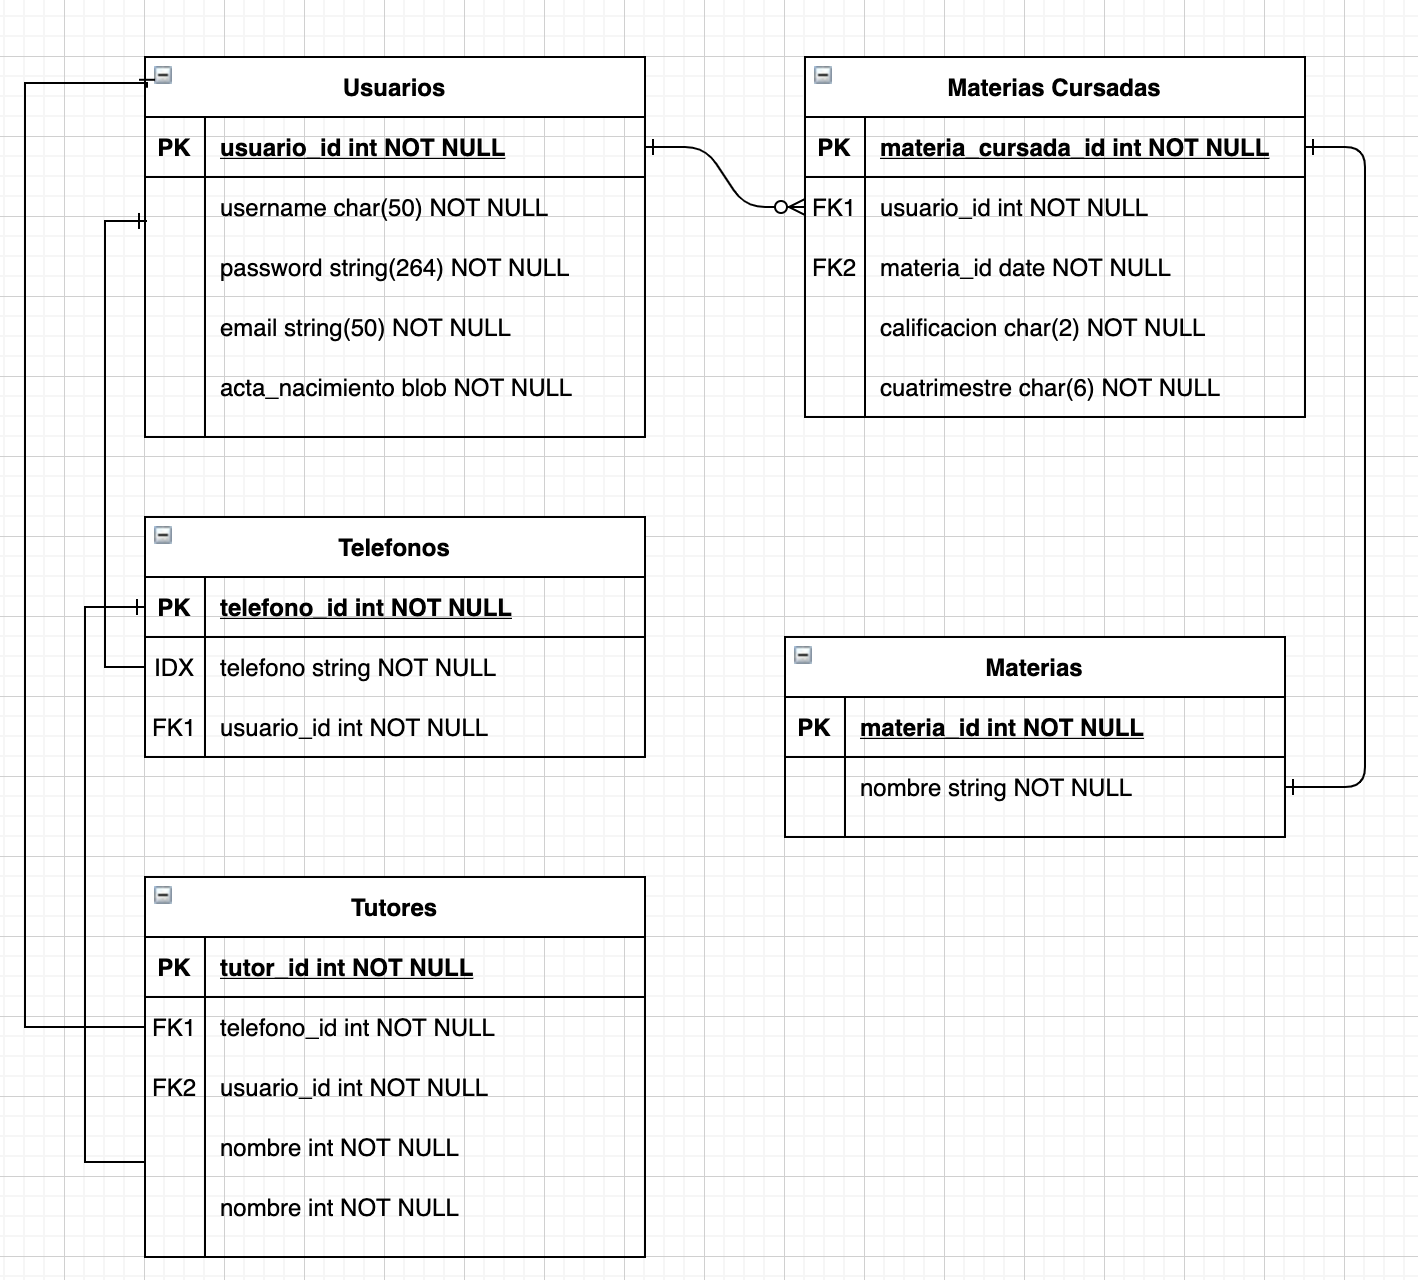
\includegraphics[scale=0.5]{{./diagrama}}
  \caption{Diagrama del modelo de datos}
  \label{fig:1}
\end{figure}

\section{Enpoints}

Todos los enpoints incluyen las operaciones \texttt{list},
\texttt{create}, \texttt{update}, \texttt{read} y \texttt{delete} a
menos que se indique explícitamene lo contrario.

\begin{itemize}
\item \texttt{/usuarios} Meta-modelo que contiene a los modelos
  \texttt{Usuarios}, \texttt{Materias Cursadas}, \texttt{Tutores} y \texttt{Teléfonos}.
\item \texttt{/usuarios/{id}/tutores} Sirve para manejar los tutores de los usuarios.
\item \texttt{/usuarios/{id}/telefonos}  Maneja los teléfonos de los usuarios.
\item \texttt{/usuarios/{id}/materias}  Manjea las materias cursadas por el alumno.
\item \texttt{/materias} Maneja las materias.

\end{itemize}
\end{document}
%%% Local Variables:
%%% mode: latex
%%% TeX-master: t
%%% End: